
%\vspace{-3mm}

\section{Experimental Setup}
%In this section we evaluate the effectiveness of our algorithm as compared to the existing methods. We start by explaining the datasets and baseline sampling algorithms. Then we provide the criteria to evaluate the competing algorithms, followed by a detailed comparative analysis. 
In this section, we describe the baseline sampling algorithms and the datasets used in our experiments.

\subsection{Sampling algorithms}
We compare \compas~ with five existing sampling methods: (i) Streaming Node (SN) \cite{ahmed2014network}, (ii) Streaming Edge (SE) \cite{ahmed2014network}, (iii) Streaming BFS (SBFS) \cite{ahmed2014network}, (iv) PIES \cite{ahmed2014network}, and (v) Green algorithm (GA) \cite{tong2016novel}. The first four algorithms are exclusively designed for streaming graphs while the last one is designed for static graphs. Note that unlike ours, none of the existing methods explicitly produce a community structure as a by-product of the sampling,
%\footnote{Although GA claims that its sample graph preserves the underlying community structure, it does not explicitly produce the community structure.}, 
and thus one needs to execute community detection algorithm separately on the sample to obtain the community structure. Therefore to evaluate the competing methods w.r.t how the underlying community structure in the sample resembles with that of the original graph, for SN, SE, SBFS and PIES we run Louvain algorithm~\cite{blondel2008fast}
\footnote{We also considered other algorithms (CNM \cite{clauset2004finding}, GN \cite{girvan2002community} and Infomap \cite{rosvall2008maps}) and found the results to be similar.} 
%\noteng{are there results on that?} \textcolor{blue}{Yes}
%} 
on each individual sample and detect the communities. In case of GA, we consider the aggregated graph and run GA to obtain the sample, and further run Louvain algorithm on the sample to detect the community structure. 
Note that although by considering the aggregated graph, GA acquires far more information of the entire graph structure, we use it as a strict baseline in this study.
%to show that the community structure obtained from \compas~is quite competitive to that obtained by running community detection on GA's sample graph.   

\begin{table}[]
\centering
\caption{Datasets used for evaluation.}
\label{tab:data}
%\begin{adjustbox}{max width=0.5\textwidth}
\begin{tabular}{l l l l l l}
\hline
Dataset  & Facebook & arxiv hep-th & Youtube   & Dblp      & LFR     \\ \hline
\# Nodes & 63,731   & 22,908       & 1,134,890 & 317,080   & 25,000  \\ 
\# Edges & 817,035  & 2,444,798    & 2,987,624 & 1,049,866 & 254,402 \\ \hline
\end{tabular}
%\end{adjustbox}
%\vspace{2mm}
\vspace{3mm}
\end{table}



%\vspace{3mm}
\subsection{Datasets}\label{sec:dataset}

We perform our experiments on following five graphs  (first two are streaming graphs, and last three are static graphs):  

(i) {\bf Facebook}~\cite{d1}, 
%\footnote{konect.uni-koblenz.de/networks/facebook-wosn-links}: 
An undirected graph where nodes (63,731) are users, and edges (817,035) are friendship links that are time-stamped;  % \TODO{Is there a ground truth community structure? Else how do you obtain communities here?} \textcolor{blue}{done}\\

(ii) {\bf arxiv hep-th:}, 
 \footnote{konect.uni-koblenz.de/networks/ca-cit-HepTh}: 
Here nodes (22,908) are authors of arXiv's High Energy Physics papers and an edge exists between two authors if they have co-authored a paper; edges (2,444,798) are time-stamped by the publication date;% \TODO{Is there a ground truth community structure? Else how do you obtain communities here?}\textcolor{blue}{done}\\ 
 
 (iii) {\bf Youtube:}, 
\footnote{snap.stanford.edu/data/com-Youtube.html}:
Nodes (1,134,890) represent Youtube users and edges (2,987,624) representing friendship.
%User created groups in the network form the ground truth community structure. There are 8,385 communities in the ground truth.\\

(iv) {\bf dblp:} 
\footnote{snap.stanford.edu/data/com-DBLP.html}:
This dataset consists of authors indexed in DBLP. The graph is same as arxiv hep-th (317,080 nodes and 1,049,866 edges);
Publication venue defines ground truth communities. There are 13,477 communities in the ground truth.

(v) {\bf LFR}~\cite{lancichinetti2008benchmark} This is a synthetic graph with underlying community structure implanted into it (Table \ref{tab:data}).
We construct the graph with 25,000 nodes, 254,402 edges and 1,834 communities.
%{\color{red} put \# of nodes and edges}
%The first three datasets were presented by Yang et.~al. in \cite{yang2015defining}.
%Although the above graphs are all static, we assign 

Since last three graphs are static, we consider that each edge arrives in a pre-decided (random) order, i.e., each edge has a (discrete) time of arrival. 
The edge ordering, as we shall see, does not influence the inferences drawn from the results.
Moreover, since first four graphs do not have any underlying ground-truth community structure, we run louvain algorithm %\cite{blondel2008fast} {\color{red} only louvain?} 
on the aggregated graph and obtain the disjoint community structure. This community structure is the best possible output that we can expect from our incremental modularity maximization method, and therefore serves as the ground-truth. 


\begin{table}
\centering
\caption{Summary of the D-statistics (the lower, the better) values of the topological measures for Facebook. Top two values for each average result is highlighted.}
\label{tab_fb}
\begin{adjustbox}{max width=\textwidth}
\begin{tabular}{c|c c c c c c c c c c c c c }
\hline
Algorithm & ID & EI & AD & FOMD & TPR & EX & CR & CON & NC & AODF & MODF & FODF & MOD \\ \hline
Compas    & 0.08   & 0.11   & 0.15   & 0.32     & 0.28    & 0.14   & 0.12   & 0.16    & 0.09   & 0.14     & 0.11     & 0.41     & 0.16    \\ 
SN        & 0.26   & 0.21   & 0.22   & 0.42     & 0.86    & 0.20   & 0.34   & 0.19    & 0.15   &  0.36    & 0.24     & 0.40     & 0.33    \\ 
SE        & 0.19   & 0.15   & 0.21   & 0.28     & 0.57    & 0.27   & 0.24   & 0.20    & 0.17   & 0.41     & 0.25     & 0.37     & 0.25    \\ 
SBFS      &  0.25  & 0.29   & 0.27   & 0.38     & 0.28    & 0.18   & 0.15   & 0.17    & 0.16   & 0.26     & 0.27     & 0.48     &  0.26   \\ 
PIES      & 0.27   &  0.28  & 0.30   & 0.31     & 0.41    & 0.17   &  0.23  &  0.21   &  0.30  & 0.35     & 0.37     &  0.29    & 0.28    \\ 
GA        & 0.14    &  0.17   &  0.21   & 0.12     &  0.09   &  0.06  & 0.09   &  0.13    & 0.15   & 0.11     &  0.07      & 0.10   & 0.12 \\ \hline
\end{tabular}
\end{adjustbox}
\vspace{3mm}
\end{table}


%\vspace{-3mm}
\section{Evaluation}
\iffalse
We design a two-fold experimental setup. First, we show how  competing sampling algorithms detect the original community structure, and second, we measure how good individual samples are w.r.t. the structural properties of the original graph. Although the primary focus of \compas~is to improve upon in the first evaluation, we also show that it is quite competitive in terms of the second evaluation.
\fi

\begin{table}
\centering
\caption{Summary of the D-statistics values of the topological measures for arxiv hep-th graph.}
\label{tab_hep-th}
\begin{adjustbox}{max width=\textwidth}
\begin{tabular}{c|c c c c c c c c c c c c c}
\hline
Algorithm & ID & EI & AD & FOMD & TPR & EX & CR & CON & NC & AODF & MODF & FODF & MOD \\ \hline
Compas    & 0.12 & 0.06 &0.09 & 0.06  &  0.14 & 0.13  &  0.10   & 0.09   & 0.07     &   0.16   &  0.06& 0.08   &  0.10   \\ 
SN        & 0.29   & 0.25   & 0.28   &  0.22    &  0.19   & 0.32   &  0.24  &  0.20   & 0.21   & 0.28     & 0.33     &   0.26   &  0.31 \\ 
SE        & 0.22   &  0.27  &  0.37  &  0.36    &  0.31   &  0.35  &  0.21  &  0.29   &  0.32  &  0.29    &  0.26    & 0.21     &  0.31   \\ 
SBFS      &  0.22  & 0.27   &  0.26  &  0.18    &   0.38  &  0.31  & 0.34    &  0.21   & 0.25   &  0.23    & 0.25     &  0.26    &  0.22   \\ 
PIES      & 0.15   &  0.21  &  0.23  &  0.27    &  0.14   & 0.24    & 0.26   & 0.23    &  0.17  & 0.21     &  0.13   &  0.19    &  0.29   \\ 
GA        &  0.11  & 0.08   & 0.12   &   0.10   & 0.08    & 0.05   & 0.06   & 0.09    &   0.06 &  0.07    &  0.04    &  0.14 &  0.06 \\ \hline
\end{tabular}
\end{adjustbox}
\vspace{3mm}
\end{table}


\begin{table}[!t]
\centering
\caption{\label{tab_yt}Summary of the $D$-statistics (the lower, the better) values of the topological measures for Youtube dataset.}
% \TODO{Provide standard deviation/error $\sigma$ for the last 4 networks.}}


\begin{adjustbox}{max width=\textwidth}
\begin{tabular}{l|c c c c c c c c c c c c c |}
\hline
Algorithm & ID & EI & AD & FOMD & TPR & EX & CR & CON & NC & AODF & MODF & FODF & MOD \\ \hline
\compas     & 0.063   & 0.051   & 0.078    & 0.057     & 0.227    & 0.082   & 0.054   & 0.091    & 0.260   & 0.073    & 0.201     &  0.121    & 0.052  \\ 
SN         & 0.164   &  0.171  & 0.471   & 0.061     & 0.542    & 0.581   & 0.112   & 0.265    & 0.064   & 0.157     & 0.182     & 0.092     &  0.216  \\ 
SE         &  0.257  & 0.244   & 0.241   & 0.501     & 0.281    & 0.098   & 0.287   & 0.087    & 0.151   & 0.097     &  0.246    &  0.093    & 0.198   \\ 
SBFS       &  0.126  & 0.131   & 0.172   &  0.106    & 0.454    & 0.145   & 0.056   & 0.165    & 0.045   &   0.257   & 0.108     & 0.076     & 0.181   \\ 
PIES       &  0.234  & 0.241   &  0.252  & 0.190    & 0.409    & 0.042   & 0.051   & 0.049    & 0.061   &      0.157 & 0.042     & 0.053     & 0.121   \\ 
GA         &   0.156 & 0.055   & 0.065   & 0.053     & 0.267    & 0.066   & 0.076   & 0.053    & 0.085   &   0.150   & 0.075     &  0.069    & 0.102   \\ \hline
\end{tabular}
\end{adjustbox}
\vspace{3mm}
\end{table}



%\subsection{Community-centric evaluation}
In this section, we list the standard metrics used to evaluate the goodness of the community structure, followed by a detailed comparison of the sampling algorithms.

 {\bf Evaluation criteria:}
To measure how sampling algorithms capture the underlying community structure, we evaluate them in two ways.  First we measure the quality of the obtained community structure based on the {\bf topological measures} defined by \cite{yang2015defining}. In particular, we look into four classes of quality scores - (i) {\em based on internal connectivity}: internal density (ID), edge inside (EI), average degree (AD), fraction over mean degree (FOMD), triangle participation ratio (TPR); (ii) {\em based on external connectivity}: expansion (EX), cut ratio (CR); (iii) {\em combination of internal and external connectivity}: conductance (CON), normalized cut (NC), maximum out-degree fraction (MODF), average out-degree fraction (AODF), flake out-degree fraction (FODF); and (iv) {\em based on graph model}: modularity (MOD).
%\footnote{See~\cite{yang2015defining} for the detailed definitions of all these metrics.}. 
Note, for every individual community we obtain a score, and therefore a distribution of scores (i.e., distribution of ID, EI etc.) is obtained for all the communities of a graph. We measure how similar (in terms of Kolgomorov-Smirnov $D$-statistics\footnote{It is defined as $D = max_x\{|f(x) - f^{'}(x)|\}$ where $x$ is over the range of the random variable, and $f$ and $f^{'}$ are the two empirical cumulative distribution functions of the data.}) these distributions are with those of the ground-truth communities. {\em The less the value of D-statistics, the better the match between two distributions}.

\begin{table}
\centering
\caption{Summary of the D-statistics values of the topological measures for Com-dblp dataset.}
\label{tab_dblp}
\begin{adjustbox}{max width=\textwidth}
\begin{tabular}{c|c c c c c c c c c c c c c}
\hline
Algorithm & ID & EI & AD & FOMD & TPR & EX & CR & CON & NC & AODF & MODF & FODF & MOD \\ \hline
Compas    & 0.13   & 0.07   & 0.13   & 0.10     & 0.12    & 0.12   & 0.11   & 0.13    & 0.11   & 0.37     & 0.05     & 0.41     & 0.16    \\ 
SN        &  0.51  & 0.60   & 0.54   & 0.11    & 0.51    & 0.12   & 0.11   & 0.37    & 0.05   & 0.11     &   0.24   & 0.11     & 0.51    \\ 
SE        &  0.51  & 0.49   & 0.48   & 0.27    & 0.24    & 0.12   & 0.13   & 0.12    & 0.11   & 0.21     & 0.12     &  0.18    & 0.23    \\ 
SBFS      &  0.34  & 0.32   & 0.41   & 0.18     & 0.40    & 0.15   & 0.13   &  0.14   & 0.18   &  0.12    &   0.34   & 0.24     & 0.11    \\ 
PIES      & 0.27   &  0.14  & 0.24   &  0.29    & 0.17    & 0.34   & 0.28   &  0.19   &  0.20  & 0.31     & 0.32     &  0.21    &  0.16   \\ 
GA        & 0.13   & 0.16   & 0.11   &  0.05    &  0.17  & 0.08   &  0.15  &  0.14   & 0.19   & 0.07     &  0.10    &  0.09    & 0.12    \\ \hline
\end{tabular}
\end{adjustbox}
\vspace{3mm}
\end{table}


%We further measure the community quality based on the ground-truth community structure. Finally, we calculate the Kolgomorov-Smirnov $D$-statistics between the community score distribution obtained from the sample and the ground truth for each individual type of score. Note that $D$-statistics is applied as a part of Komogorov-Smirnov test to reject the null hypothesis. Here we use it to measure the agreement between the two distributions. 

As a second level of evaluation, we use the {\bf community validation metrics} --  Purity~\cite{manning2008introduction}, Normalized Mutual Information (NMI)~\cite{danon2005comparing} and Adjusted Rand Index (ARI)~\cite{hubert1985comparing} to measure the similarity between the ground-truth and the obtained community structures. {\em The more the value of these metrics, the higher the similarity.}
\if{0}
\begin{table*}[!t]
\centering
\caption{\label{g_metric_alg}Purity (PU), NMI and ARI values between the ground-truth and community structure obtained from individual sampling algorithms for all datasets.}
\scalebox{0.7}{
\begin{tabular}{l |>{\columncolor[gray]{0.8}} c>{\columncolor[gray]{0.8}}  c>{\columncolor[gray]{0.8}}  c|  c  c  c| ccc|ccc|ccc|>{\columncolor[gray]{0.8}}c>{\columncolor[gray]{0.8}}c>{\columncolor[gray]{0.8}}c}
\hline
\multirow{2}{*}{{\bf Dataset}} & \multicolumn{3}{c|}{{\bf \compas}} & \multicolumn{3}{c|}{{\bf SN}} & \multicolumn{3}{c|}{{\bf SE}} & \multicolumn{3}{c|}{{\bf SBFS}} & \multicolumn{3}{c|}{{\bf PIES}} & \multicolumn{3}{c}{{\bf GA}} \\\cline{2-19}
   & \multicolumn{1}{c}{PU} & \multicolumn{1}{c}{NMI} & \multicolumn{1}{c|}{ARI} & PU & NMI & ARI &PU & NMI & ARI &PU & NMI & ARI &PU & NMI & ARI & \multicolumn{1}{c}{PU} & \multicolumn{1}{c}{NMI} & \multicolumn{1}{c}{ARI} \\\hline
Facebook	  & 0.71 & 0.52 & 0.47	 & 0.43&0.34&0.26  & 0.39&0.28&0.12  &  0.53&0.41&0.18  & 0.57&0.48&0.36  & 0.76&0.61&0.52 \\
hep-th		  &	0.69&0.51&0.38 & 0.39&0.32&0.19 & 0.29&0.21&0.12 & 0.42&0.36&0.25  & 0.48&0.39&0.31 & 0.74&0.68&0.57\\
youtube		      & 0.83&0.72&0.67	 &  0.52&0.49&0.36 & 0.48&0.33&0.28  &  0.63&0.58&0.47 & 0.56&0.51&0.41  & 0.86&0.77&0.71 \\
Dblp		  &	0.72&0.65&0.58 & 0.32&0.28&0.21  & 0.29&0.21&0.16  & 0.66&0.57&0.32  & 0.48&0.39&0.31  & 0.79&0.69&0.52 \\
LFR		  & 0.76&0.69&0.55	 & 0.35&0.29&0.21  & 0.56&0.32&0.29  & 0.49&0.38&0.26  & 0.42&0.31&0.28  &  0.81&0.72&0.67 \\\hline
Average & 0.74 & 0.61 & 0.53 & 0.40 & 0.34 & 0.24 & 0.40 & 0.27 &0.19 & 0.54 & 0.46 & 0.29 & 0.50 & 0.41 & 0.33 & 0.79 & 0.69 & 0.59   \\
\hline
\end{tabular}}
%\vspace{-5mm}
\end{table*}
\fi
%\vspace{-3mm}

\begin{table}
\centering
\caption{Summary of the D-statistics values of the topological measures for LFR graph.}
\label{tab_lfr}
\begin{adjustbox}{max width=\textwidth}
\begin{tabular}{c|c c c c c c c c c c c c c}
\hline
Algorithm & ID & EI & AD & FOMD & TPR & EX & CR & CON & NC & AODF & MODF & FODF & MOD \\ \hline
Compas    &  0.16  &  0.23  &  0.18  &  0.12    &  0.08   & 0.20   &  0.24  &  0.13   & 0.21   &  0.28    &  0.27    &   0.15   & 0.09    \\ 
SN        &  0.21  &  0.26  &  0.17  &  0.29    &  0.14   & 0.37   & 0.27   & 0.33    &  0.28  &  0.32    & 0.25     & 0.40     &  0.22   \\ 
SE        & 0.32   & 0.36   &  0.41  &   0.46   &   0.23  & 0.31   & 0.45   &  0.28   & 0.19   &   0.38   &  0.18    &  0.26    & 0.33    \\ 
SBFS      &  0.32  &  0.15  &  0.20  &  0.12    &  0.35   & 0.37   & 0.26   &  0.29   & 0.37   &   0.09   & 0.25     &  0.30    & 0.18    \\ 
PIES      & 0.38   & 0.18   &  0.19  &  0.32    &  0.23   &  0.26  & 0.28   &  0.21   & 0.25   & 0.20     & 0.34     &  0.24    &  0.24   \\ 
GA        &  0.18  &  0.27  & 0.11   & 0.12     &  0.07   & 0.12   &  0.05  &  0.06   & 0.14   &  0.08    &  0.21    &  0.17    & 0.14    \\ \hline
\end{tabular}
\end{adjustbox}
\vspace{3mm}
\end{table}

{\bf Parameter estimation}:
As reported in Section~\ref{algorithm},~\compas consists of two parameters: (i) $\alpha$ (initial fraction of nodes inserted), (ii) $n_d$ (length of the buffer).
%In Figures \ref{param_est}(a) and \ref{param_est}(b) we plot the average  $D$-statistics for different values of $\alpha$ and $n_d$ respectively. 
We observe that $D$-statistics is initially high and reduces as we increase $\alpha$ (Figures \ref{param_est}(a)). This is because for low $\alpha$, the community structure obtained initially by running a community-detection algorithm (Step 12 in Algorithm 1) is coarse. For large values of $\alpha$ even though initial community structure obtained is good, it is not allowed to evolve much. Similarly, in Figure~\ref{param_est}(b), given a small buffer size several nodes mostly arriving once would be added to the sample leading to formation of pendant vertices. As we increase the buffer size \compas~performs better till a certain point, after which the improvement is negligible. Since we are interested in using minimum space we fix $n_d$ at $0.0075 n$. Similarly $\alpha$ is set to $0.4$. 
%Thus, for the rest of the experiments we set $\alpha$ to $0.5$ and $n_d$ to $0.0075n$ unless otherwise specified. 
We also set $n$ to $0.4|V|$ as default (see Section \ref{sec:effect} for different values of $n$). Further note that apart from Louvain we also consider other algorithms (CNM~\cite{clauset2004finding}, GN~\cite{girvan2002community} and Infomap~\cite{rosvall2008maps}) for obtaining the initial community structure. 
%{\color{red} may be Infomap, then remove "modularity optimization"}. 
The average $D$-statistics values (calculated for LFR) across all the quality scores for Louvain, CNM, GN and Infomap are respectively \textbf{0.182}, \textbf{0.191}, \textbf{0.216} and \textbf{0.197}. 
Above results indicate that \compas~ is independent of the community detection algorithm used initially and we thus stick to Louvain for evaluation.

%\vspace{-2mm}
\begin{figure}[!h]
\centering
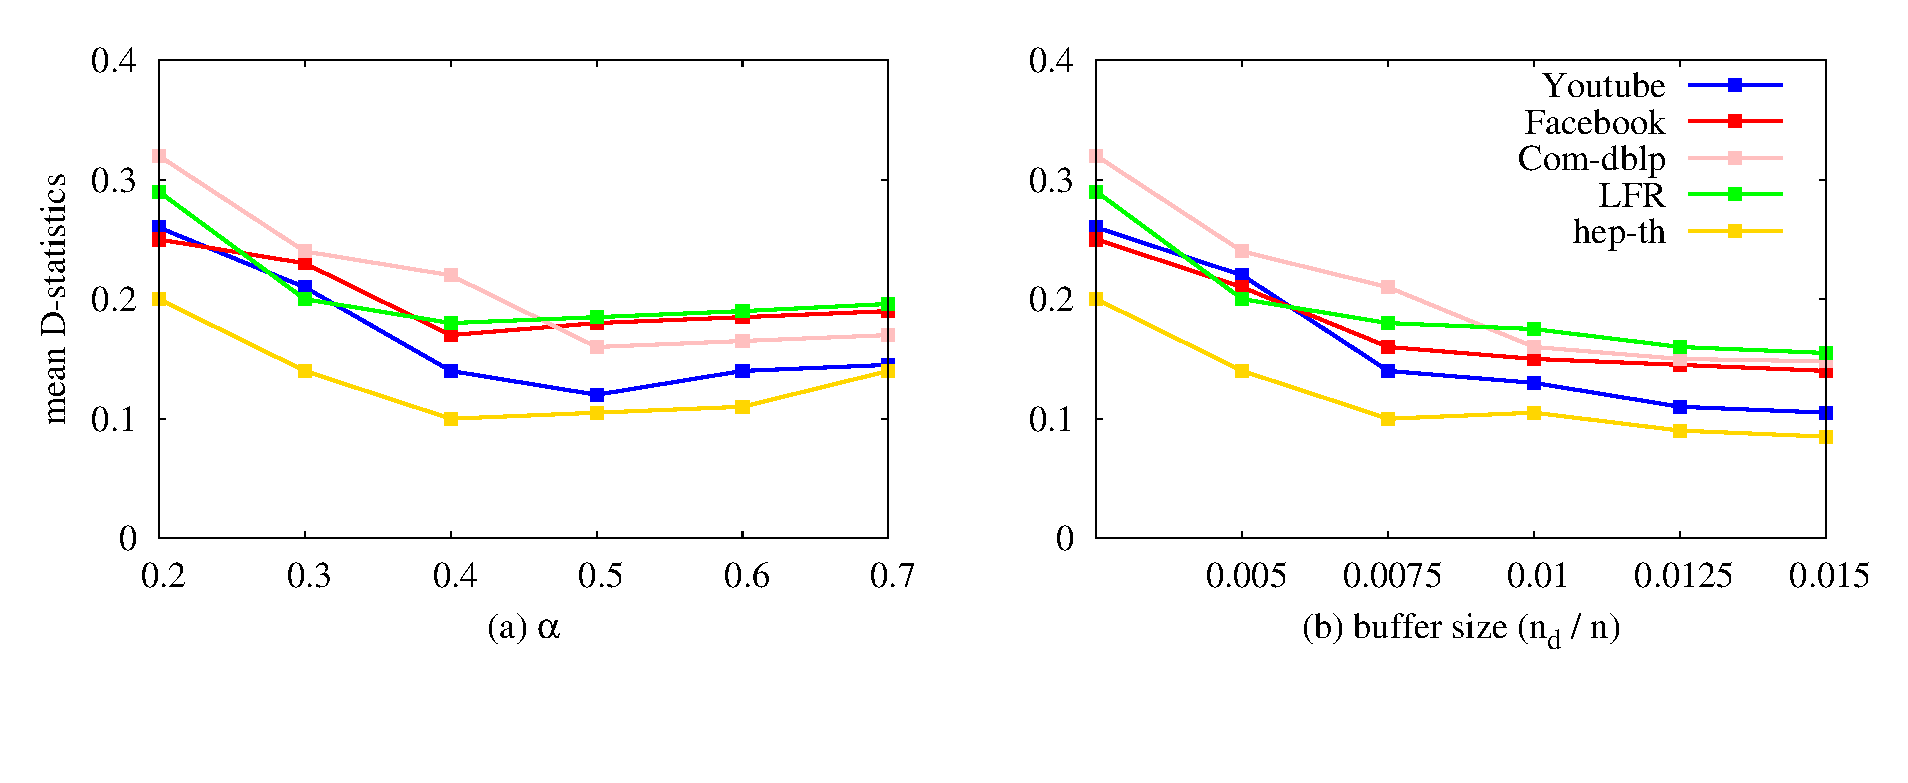
\includegraphics[width=\columnwidth]{./texfiles/Chapter_2/figures/param_estimate.eps}
%\vspace{-12mm}
\caption{\label{param_est}Average $D$-statistics value across all the topological measures.}
\vspace{3mm}
%\vspace{-3mm}
\end{figure}


\iffalse
\begin{table}[!t]
\centering
\caption{\label{g_metric_alg}NMI between the ground-truth and community structure obtained from individual sampling algorithms for all datasets.}
%\scalebox{0.8}{
\begin{tabular}{l cccccc}
\hline
\multirow{1}{*}{{\bf Dataset}} & \multicolumn{1}{c}{{\bf \compas}} & \multicolumn{1}{c}{{\bf SN}} & \multicolumn{1}{c}{{\bf SE}} & \multicolumn{1}{c}{{\bf SBFS}} & \multicolumn{1}{c}{{\bf PIES}} & \multicolumn{1}{c}{{\bf GA}} \\\hline
Facebook	  & 0.52 & 0.34 & 0.28&0.41&0.48&0.61\\
hep-th		  &0.51&0.32&0.21&0.36&0.39&0.68\\
Youtube		      &0.72&0.49&0.33&0.58&0.51&0.77 \\
dblp		  &0.65&0.28&0.21&0.57&0.39&0.69 \\
LFR		  &0.69&0.29&0.32&0.38&0.31&0.72\\\hline
Average & {\bf 0.61}  & 0.34 & 0.27 & 0.46  & 0.41 & {\bf 0.69}    \\
\hline
\end{tabular}
%\vspace{4mm}
\end{table}
\fi
\begin{table}[!t]
\centering
\caption{\label{g_metric_alg}Purity (PU), NMI and ARI values between the ground-truth and community structure obtained from individual sampling algorithms for all datasets.}
\scalebox{0.68}{
\begin{tabular}{l |>{\columncolor[gray]{0.8}} c>{\columncolor[gray]{0.8}}  c>{\columncolor[gray]{0.8}}  c|  c  c  c| ccc|ccc|ccc|>{\columncolor[gray]{0.8}}c>{\columncolor[gray]{0.8}}c>{\columncolor[gray]{0.8}}c}
\hline
\multirow{2}{*}{{\bf Dataset}} & \multicolumn{3}{c|}{{\bf \compas}} & \multicolumn{3}{c|}{{\bf SN}} & \multicolumn{3}{c|}{{\bf SE}} & \multicolumn{3}{c|}{{\bf SBFS}} & \multicolumn{3}{c|}{{\bf PIES}} & \multicolumn{3}{c}{{\bf GA}} \\\cline{2-19}
   & \multicolumn{1}{c}{PU} & \multicolumn{1}{c}{NMI} & \multicolumn{1}{c|}{ARI} & PU & NMI & ARI &PU & NMI & ARI &PU & NMI & ARI &PU & NMI & ARI & \multicolumn{1}{c}{PU} & \multicolumn{1}{c}{NMI} & \multicolumn{1}{c}{ARI} \\\hline
Facebook	  & 0.71 & 0.52 & 0.47	 & 0.43&0.34&0.26  & 0.39&0.28&0.12  &  0.53&0.41&0.18  & 0.57&0.48&0.36  & 0.76&0.61&0.52 \\
hep-th		  &	0.69&0.51&0.38 & 0.39&0.32&0.19 & 0.29&0.21&0.12 & 0.42&0.36&0.25  & 0.48&0.39&0.31 & 0.74&0.68&0.57\\
youtube		      & 0.83&0.72&0.67	 &  0.52&0.49&0.36 & 0.48&0.33&0.28  &  0.63&0.58&0.47 & 0.56&0.51&0.41  & 0.86&0.77&0.71 \\
Dblp		  &	0.72&0.65&0.58 & 0.32&0.28&0.21  & 0.29&0.21&0.16  & 0.66&0.57&0.32  & 0.48&0.39&0.31  & 0.79&0.69&0.52 \\
LFR		  & 0.76&0.69&0.55	 & 0.35&0.29&0.21  & 0.56&0.32&0.29  & 0.49&0.38&0.26  & 0.42&0.31&0.28  &  0.81&0.72&0.67 \\\hline
Average & 0.74 & 0.61 & 0.53 & 0.40 & 0.34 & 0.24 & 0.40 & 0.27 &0.19 & 0.54 & 0.46 & 0.29 & 0.50 & 0.41 & 0.33 & 0.79 & 0.69 & 0.59   \\
\hline
\end{tabular}}
\vspace{3mm}
\end{table}
 {\bf Comparison of sampling algorithms}:
We start by measuring the similarity between the obtained and the ground-truth community structures using topological measures. In tables~\ref{tab_fb},~\ref{tab_hep-th},
~\ref{tab_yt},~\ref{tab_dblp} and ~\ref{tab_lfr} 
we summarize the $D$-statistics values of all the scoring functions for Facebook, arxiv hep-th, Youtube, dblp and LFR datasets respectively. 
%for the other graphs we only present the average value (and standard deviation) across the $D$-statistics for different topological 
%measures (detailed results on other datasets can be accessed in  \cite{si}). 
\iffalse\TODO{For these networks we MUST report standard deviation/error}.\fi 
Clearly~\compas~outperforms all the streaming algorithms across different datasets. GA performs better than~\compas~since it has in its 
consideration the whole graph to obtain the sample. However, we stress that even with {\em minimal community information to start with} and 
{\em no subsequent community detection in the later steps}, we are able to reach very close to GA as well as to the ground-truth.

Further we find \compas~is the second ranked algorithm after GA with an average 
(over all datasets) purity, NMI and ARI of \fbox{{\bf 0.74}, {\bf 0.61} and {\bf 0.53}} respectively (see table \ref{g_metric_alg} for detailed results). 
%(see Table \ref{g_metric_alg}  for NMI, details in \cite{si}).
\iffalse As a second level of evaluation, we further calculate three validation metrics -- purity, NMI and ARI  between the ground-truth and the obtained community structure for all the algorithms . Once again we observe that \\ \fi


{\bf Comment on edge-density of the sample}: 
Note that \compas~ is node-based, i.e., sample size is controlled by the number of nodes, and we at any point do not limit the number of edges in the sample ($e_{s}$). We compare the number of edges in the sample against that in the subgraph induced by the nodes in the obtained sample ($e_{p}$). 
We observe that on average our sample consists of only $\sim71$\% of the edges in the induced subgraph across all the datasets. 
%\iffalse\TODO{Sandipan: I had initially added a plot but decided against putting it as I felt it was not providing any extra information.}\fi
%which is followed by SBFS, PIES, SN and SE.
\iffalse
\subsection{Graph-centric evaluation}
\label{graph_evaluation}
We further evaluate our sample in terms of three graph properties mentioned in \cite{ahmed2014network}: (i) degree distribution (Degree), (ii) clustering coefficient distribution (CC), (iii) top 100 eigen value distribution (EV). 
Table \ref{graph_prop} reports the $D$-statistics values between the distributions of the original graph and those obtained from the sample (see more results in \cite{si}). For all the datasets, we observe that \compas~is within top three ranks in terms of low $D$-statistics, in many cases, also beating the strict baseline GA. This indicates that \compas~ also preserves general graphs properties in the sample.

\vspace{-2mm}
\begin{table}[!h]
\centering
\caption{Summary of $D$-statistics for different graph properties. For Youtube we present all the results, while for the rest we provide only average $D$-statistics (top three results in each average case are highlighted).}
\label{graph_prop}
\begin{adjustbox}{max width=\columnwidth}
\begin{tabular}{l|c c c |c|c|c|c|c}
\hline
  \multirow{2}{*}{Algorithm}         & \multicolumn{4}{c|}{Youtube}     & Facebook & Com-dblp & LFR     & hep-th  \\ \cline{2-9}
& Degree & CC & EV & Average & Average  & Average  & Average & Avearge \\ \hline
\compas    &   0.083     & 0.105   & 0.42     &  {\bf 0.20}       &  {\bf 0.17}        &  {\bf 0.16}       & {\bf 0.28}        & {\bf 0.18}       \\ 
SN        &    0.076    & 0.108   &  0.54     &  0.24             &   0.36             &  0.24             & 0.34              &  0.23       \\ 
SE        &    0.114    & 0.195   &  0.39     &  0.23             &   0.48             &  0.28             & 0.39              &  0.27       \\ 
SBFS      &    0.105    & 0.172   &  0.32     &  {\bf 0.19}       &   {\bf 0.28}       &  {\bf 0.13}       & {\bf 0.26}        & {\bf 0.19}       \\ 
PIES      &    0.046    &  0.129  &  0.38     &  {\bf 0.18}       &   {\bf 0.16}       &  0.21             & {\bf 0.28}        & {\bf 0.16}        \\ 
GA        &    0.218    &  0.063  &  0.46     &  0.24            &   0.35             &  {\bf 0.12}       & 0.32              &  0.20       \\ \hline
\end{tabular}
\end{adjustbox}
\vspace{-1mm}
\end{table}
\fi
%\vspace{-2mm} 

{\bf Effect of edge ordering and sample size:}
\iffalse As mentioned in Section \ref{sec:dataset}, we artificially imposed an edge ordering for two static graphs -- Youtube and LFR.\fi In this section, we show that most of our inferences are valid irrespective of any edge ordering. To do so, we randomly pick one pair of edges and swap their arrival time. We repeat it for 20\% of  edges present in each static graph. The entire experiment is repeated $20$ times and the average value is reported. Figure \ref{param_est_1}(a) shows that for the Youtube graph edge ordering does not affect   the final  sample much (the pattern is same for LFR graph, see \cite{si}).
%\TODO{Mention how you obtained the ordering each time? Is it different random order or is there some strategic order also. You should make it explicit and say that~\compas~is tolerant to only these orders. DONE} 
%\textcolor{blue}{To obtain arrival sequences we consider two edges and swap their arrival times. This we do for 20\% of the total edges in the original network.
Lastly, we present the effect of sample size ($n$) on the obtained community structure. We plot average $D$-statistics values across all the topological measures for all the algorithms on Youtube  (see others in \cite{si}) as a function of $n$ (Figure \ref{param_est_1}(b)). As expected, with the increase of $n$ we obtain better results. Interestingly, for~\compas~and GA, the pattern remains consistent compared to others.\\

%\vspace{-5mm}
\begin{figure}[!h]
\centering
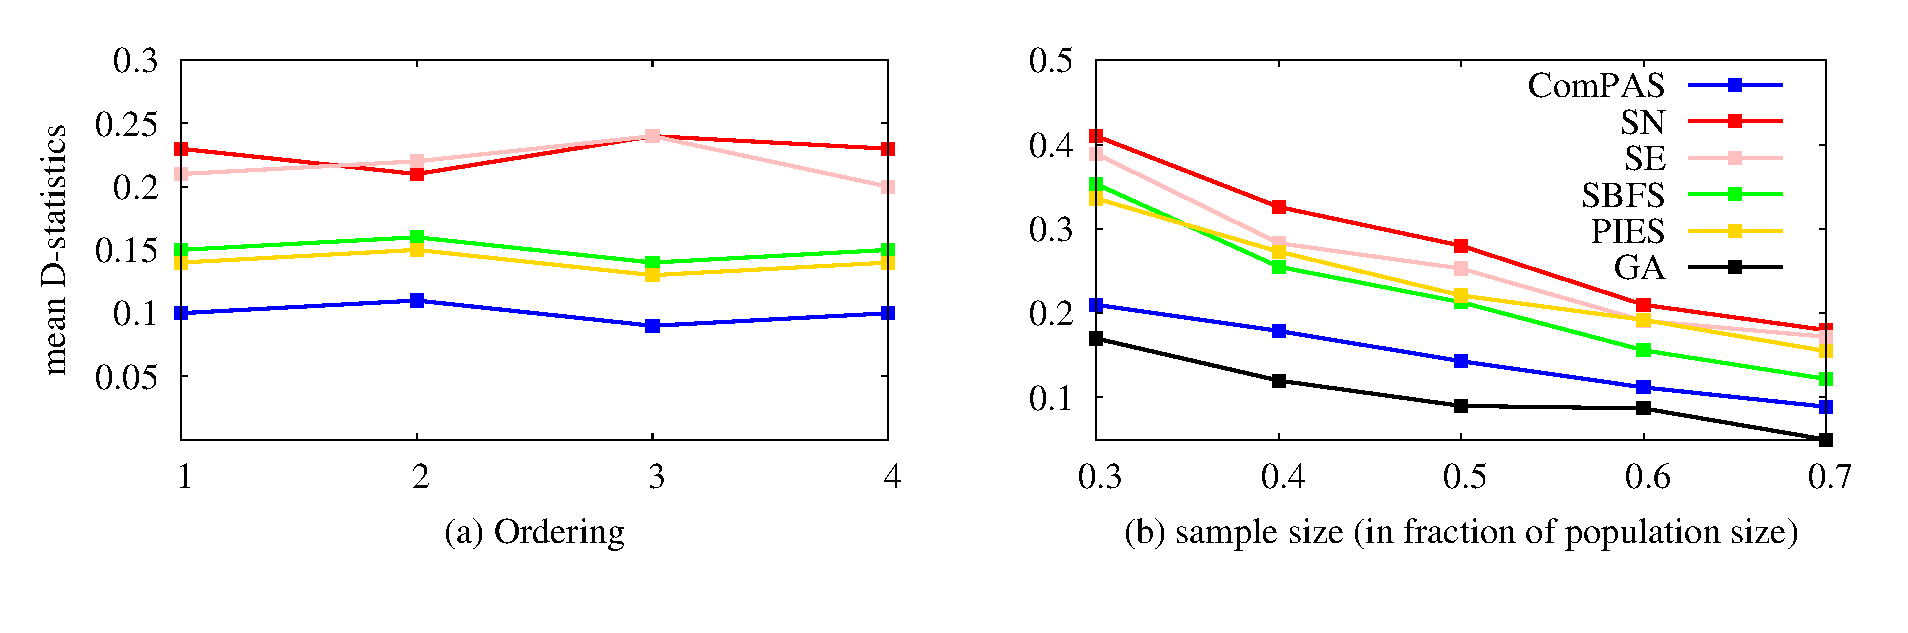
\includegraphics[width=\columnwidth]{./texfiles/Chapter_2/figures/param_estimate_1.eps}
%\vspace{-10mm}
\caption{\label{param_est_1}Average $D$-statistics across all the topological measures for (a) different edge ordering and (b) sample size ($n$) of the Youtube graph.}
%\vspace{-4mm}
\end{figure}


%\if{0}

%\fi




